\documentclass[8pt]{extarticle}

% set document information
\title{ChipMulticoreProcessors}
\author{Fabian Olbert}                    % optional, delete if unchanged
% \myemail{info@latex4ei.de}           % optional, delete if unchanged
% \mywebsite{www.latex4ei.de}          % optional, delete if unchanged
% \usepackage{float}


\usepackage{amsmath}
\usepackage{xcolor}
% \usepackage{sectsty}
\usepackage{multicol}
\usepackage[a4paper, landscape, margin=0.5cm]{geometry}
\usepackage{microtype}
\usepackage{ulem}
\usepackage{listings}
\usepackage{graphicx}


\lstset{
  basicstyle=\ttfamily\footnotesize, % Smaller font for listings
  breaklines=true,                 % Allow lines to break
  captionpos=b,                    % Caption at the bottom
  numbers=left,                    % Line numbers on the left
  numberstyle=\tiny\color{gray},   % Style for line numbers
  showstringspaces=false           % Don't show spaces in strings with special char
}


% In your preamble
\definecolor{catBlue}{HTML}{0065bd}
\definecolor{nordicRed}{HTML}{FFFDE7	}

\makeatletter\let\inserttitle\@title\makeatother
\makeatletter\let\insertauthor\@author\makeatother

\usepackage{titlesec}

\titleformat{\section}[runin] % Command to customize
{\large\scshape\color{catBlue}} % Format for the whole heading (font, size, weight, color)
{\thesection  \quad} % The label (section number followed by a period)
{0.1cm } % Horizontal separation between label and title text
{} % Code to appear before the title text (e.g., \MakeUppercase)
[]

\titlespacing*{\section} % Use * version to affect first paragraph after heading too
{0pt} % Left margin (indentation of the heading itself)
{1.5ex plus 0.5ex minus 0.2ex} % Space BEFORE the heading (stretchable/shrinkable)
                                 % Default is often around 3.5ex plus 1ex minus .2ex
{0.5ex plus 0.2ex} % Space AFTER the heading (stretchable/shrinkable)
                     % Default is often around 2.3ex plus .2ex

\titleformat{\paragraph}[runin]
{\normalfont\scshape\ttfamily\color{black}}{}{0cm}{}

\titlespacing*{\paragraph}{0ex}{1.5ex}{3ex}

% custom commands:
\newcommand{\coloreq}[1]{\colorbox{nordicRed}{\(\displaystyle #1\)}}



% ======================================================================
% Begin
% ======================================================================
\begin{document}
\setlength{\columnseprule}{0.2pt}

\begin{multicols*}{4}


% ---- apply title
\noindent
{\Large\scshape\color{catBlue}\inserttitle} % Large, bold title
  %{\par\noindent\small\color{catBlue}\insertauthor} % Author name

\section{Overview}


\paragraph{dynamic power dissipation} \coloreq{{P_{dyn} = \alpha C f V_{dd}^2}}

\paragraph{processor coefficient} \coloreq{\delta_0 = \alpha \cdot C}

\paragraph{power density} \coloreq{ Pd = \frac{P_{dyn}}{area \cdot N_{cores}} \quad [\frac{W}{mm^2}]}

\paragraph{instructions per second} \mbox{} \\ 
\indent \coloreq{ IPS = IPC \cdot f_{clk} \quad [\text{MIPS or GIPS}]}

\paragraph{propagation delay} \coloreq{t_{pd} \sim C \cdot \frac{1}{V_{dd} - V_t}} 

\paragraph{calculte new voltage} \coloreq{t_{pd,1} = N_{cores} \cdot t_{pd,N}}

\paragraph{amdahl's law} parallel execution time: \newline 
\indent\coloreq{T' = (s + \frac{p}{N_p}) T}


\section{Synchronization}

\paragraph{Critical Sections}...

\paragraph{Mutual Exclusion}...

\paragraph{Basic Lock Propertis}...
  \begin{enumerate}
    \item Mutual exclusion
    \item Deadlock-freedom (liveness)
    \item Starvation-freedom
  \end{enumerate}

\paragraph{Atomicity}...

maybe add different lock approaches

\paragraph{Spinlocks vs. Blocking}...

\paragraph{Semaphore}...

\paragraph{Monitors}...

\paragraph{Signaling and Waiting}...

\paragraph{Condition Variables}
\begin{enumerate}
  \item[$\bullet$] \texttt{wait()}: append thread to queue of waiting threads, suspend thread
  \item[$\bullet$] \texttt{signal()}: pop thread from queue, reactivate thread
  \item[$\bullet$] \texttt{broadcast()}: reactivate all threads in queue
\end{enumerate}   

\paragraph{Peterson Lock}
add solution to thre thread solution

\paragraph{multi thread solution} filter lock or baker's lock

\paragraph{Barriers}...

\paragraph{Coarse-grained Locking} ...

\paragraph{Fine-grained Locking} a
\paragraph{Compare-and-swap} read value, if value matches compare value: swap, if it does not match: leave old value, return value  

\begin{lstlisting}[language=c, numbers=none]
  int cas(int* addr,
          int compare,
          int swap) {
    int tmp=*addr;
    if (tmp==compare) {
      *addr=swap;
    }
    return tmp;
  } 
\end{lstlisting} %s

\begin{lstlisting}[language=c, numbers=none]
  void push(elem *E) {
    elem *tmp;
    do {
      tmp=top->next;
      E->next=tmp;
    } while (CAS(&top->next,tmp,E)!= tmp);
  }
\end{lstlisting} %s

\paragraph{ABA problem}...

\paragraph{Approaches to solve the ABA problem}... 

\paragraph{Load-Linked(LL)/Store-Conditional(SC)}Load-link returns the current value of a memory location, while a subsequent store-conditional to the same memory location will store a new value only if no updates have occurred to that location since the load-link.


\begin{center}
  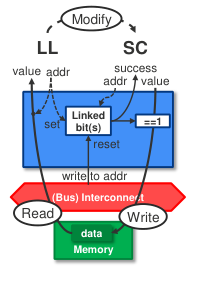
\includegraphics[width=0.4\linewidth]{img/load-linked_overview.png}
  \label{fig:load-linked_overview}
\end{center}

pseudocode:

\begin{lstlisting}[language=c, numbers=none]
  int linked[] = { 0 };
  int ll(int *addr){
    linked[addr] = 1;
    return *addr;
  }

  void on_anymem_write_access(int *addr){
    linked[addr] = 0;
  }

  bool sc(int *addr, int value) {
    if (linked[addr] == 1) {
      *addr = value;
      linked[addr] = 0;
      return true;
    }
    return false;
  }
\end{lstlisting} %s

usage stack:

\begin{lstlisting}[language=c, numbers=none]
  elem* pop() {
    elem *ret,*nxt;
    do {
      ret=LL(top->next);
      nxt=ret->next;
    } while (!SC(&top->next,nxt));
    return ret;
  }
\end{lstlisting} %s



\paragraph{Problem Set of Synchronization Primitives}...

\paragraph{Transactional Memory} Define sequence of instructions as an atomic block.

\begin{lstlisting}[language=c, numbers=none]
void insert(elem *E, elem* after) {
  atomic {
    E->next = after->next;
    after->next = E;
  }
}

void remove(elem *E) {
  atomic {
    elem *prev=get_prev(E);
    prev->next=E->next;
  }
}
\end{lstlisting} %s


\section{Memory}

\paragraph{Memory Wall} Access latencies of (DRAM) memoreis did not improve the same way as Processors did. This leads to a gap between the invrease of CPU and memory performance of around 30\% per year.

\paragraph{Performance of Memory Subsystem without Cache} 
$CPI_{mem} = CPI_{mem,instr} + CPI_{mem,d}$ \\
$r_{acc} = r_{acc,inst} + r_{acc,data}$

\paragraph{Performance of Memory Subsystem with Cache} 
$CPI = CPI_{cpu} + CPI_{mem}$ \\
$CPI_{mem} = r_{acc}((T_{cache} \cdot f_{cpu}) + r_{miss} \cdot T_{DRAM} \cdot f_{cpu})$ \\
$CPI_{mem} = r_{acc}(CPI_{cache}) + r_{miss} \cdot CPI_{DRAM})$

\paragraph{Memory Hierarchy} Up to 3 levels: L1, L2, L3. Performance/cost optimization: fast small caches nearer to the core, bigger caches with higher associativity (increased hit rate but higher latency) and thus lower miss rate far from core. L1 cache is part of the core.

\noindent
$CPI_{mem} = r_{acc} \cdot f_{cpu}(r_{miss1} \cdot (T_{C2} + r_{miss2} \cdot (T_{C3} + r_{miss3} \cdot T_{DRAM})))$

\paragraph{SDRAM Read Access Operation} \mbox{}   %s 

\noindent
Bandwidth metrics:

\noindent
$BW_{peak} = f_{mem} \cdot w$

\noindent
$BW_{burst,n} = 
\begin{cases}
\frac{f_{\text{mem}} \cdot w \cdot n}{t_{RC}} & , n \leq t_{RC} - t_{\text{mem\_acc}} \\[2ex]
    \frac{f_{\text{mem}} \cdot w \cdot n}{t_{\text{mem\_acc}} + (n-1)} & , \text{else}
\end{cases}$
$BW_{single word} = \frac{f_{mem} \cdot w}{t_{RC}}$

\noindent
Latency metrics:

\noindent

$t_{memAcc} = t_{RCD} + CL$

$t_{RC} = t_{RAS} + t_{RP}$

\paragraph{Memory BW Increase through}

\begin{enumerate}
  \item[$\bullet$] more memory channels
  \item[$\bullet$] 3D IC stacking
\end{enumerate}


\paragraph{Cache Coherency} Properties
\begin{enumerate}
  \item[$\bullet$] 
  \item[$\bullet$] 
\end{enumerate}

\subsection{Snoop-based Cache Coherency}

\paragraph{example coherency protocl (MSI)}

maybe insert state diagram

\paragraph{example coherency protocl (MESI)}

\begin{center}
  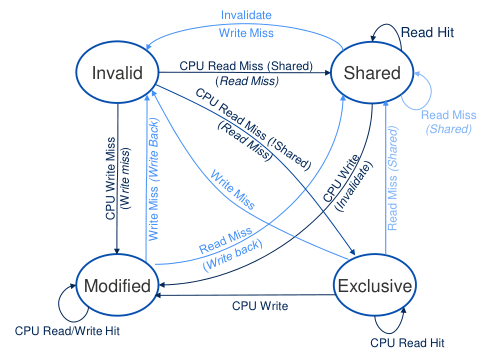
\includegraphics[width=0.8\linewidth]{img/MESIStates.png}
  \label{fig:mesistates}
\end{center}

\paragraph{Shared Memory without a shared bus}

\subsection{Directory-based Cache Coherency}

\subsection{Consistency Models}

\begin{enumerate}
  \item[$\bullet$] Sequential Consistency
  \item[$\bullet$] Relaxed Consistency
  \item[$\bullet$] Weak Consistency 
  \item[$\bullet$] Release Consistency
\end{enumerate}




\end{multicols*}

\end{document}
